\documentclass{article}

\usepackage{amsmath}
\usepackage{amsfonts}
\usepackage{graphicx}
\usepackage{stmaryrd}
\usepackage{geometry}
\usepackage{float}
\usepackage{pdfpages}

\geometry{hmargin = 2.5cm, vmargin = 1.5cm}

\title{IEOR 263A : Homework 8}
\author{Arnaud Minondo}
\begin{document}
\maketitle
\section*{Problem 6.1 :}
$\forall (p,q)\in\mathbb{N}^2$ the states are : $(p,q)$. $P_{(p,q)(p+1,q)} = \frac{1}{2}$ and $P_{(p,q)(p,q+1)} = \frac{1}{2}$ with a rate $v_{(p,q)} = (p+q)\lambda$
\section*{Problem 6.6 :}
\textbf{a.} Let $\forall i \in \mathbb{N}$, $T_i$ be the time to go from state $i$ to state $i+1$, $\mathbb{E}(T_{04}) = \sum\limits_{j=0}^3\mathbb{E}(T_{j})$ with $\forall j\in\mathbb{N}^*$, $\mathbb{E}(T_j) = \frac{1}{\lambda_j}+\frac{\mu_j}{\lambda_j}\mathbb{E}(T_{j-1}) = \frac{1}{(j+1)\lambda}+\frac{j\mu}{(j+1)\lambda}\mathbb{E}(T_{j-1})$ and $\mathbb{E}(T_0) = \frac{1}{\lambda}$.
Finally : $$\boxed{\mathbb{E}(T_{04}) = \sum\limits_{j=0}^3\mathbb{E}(T_{j})}$$
\\\\
\textbf{b.} Same as before : 
$$\boxed{\mathbb{E}(T_{25}) = \sum_{j=2}^4\mathbb{E}(T_j)}$$
\\\\
\textbf{c.} We use the formula : $\forall i\in\mathbb{N}^*\mathbb{V}(T_i) = \dfrac{1}{\lambda_i(\lambda_i+\mu_i)}+\dfrac{\mu_i}{\lambda_i}\mathbb{V}(T_{i-1})+\dfrac{\mu_i}{\mu_i+\lambda_i}(\mathbb{E}(T_i)+\mathbb{E}(T_{i-1}))^2$ and $\mathbb{V}(T_0) = \frac{1}{\lambda^2}$. With the independence between $T_i$ and $T_j$ $\forall(i,j)\in\mathbb{N}^2, i\neq j$ we have : $$\boxed{\mathbb{V}(T_{04}) = \sum_{j=0}^3\mathbb{V}(T_j) \text{ and }\mathbb{V}(T_{25}) = \sum_{j=2}^5\sum_{j=2}^4\mathbb{V}(T_j)}$$
\\\\
\textbf{d.} This is quite different as you have infinite possible ways, we notice that $\mathbb{E}(T_{40}) = \mathbb{E}(T_{43})+\mathbb{E}(T_{32})+\mathbb{E}(T_{21})+\mathbb{E}(T_{10})=4\mathbb{E}(T_{10})$ and as $\mathbb{E}(T_{10}) = \dfrac{1}{\mu-\lambda}$ then $$\boxed{\mathbb{E}(T_{40}) = \dfrac{4}{\mu-\lambda}}$$
\section*{Problem 6.15 :}
\textbf{a.} An equivalent Markov chain to the problem would be defined by the transition matrix $P = \left(\begin{array}{cccc}
    \frac{4}{7}&\frac{3}{7}&0&0\\
    \frac{2}{7}&\frac{2}{7}&\frac{3}{7}&0\\
    0&\frac{4}{7}&0&\frac{3}{7}\\
    0&0&\frac{4}{7}&\frac{3}{7}\\
\end{array}\right)$
\\
Let $\pi = (\pi_0,\pi_1,\pi_2,\pi_3)$ be the stationary distribution. On the long run the proportion of clients lost is equal to $\dfrac{\pi_3\lambda}{\pi_0\lambda+\pi_1\lambda+\pi_2\lambda+\pi_3\lambda} = \pi_3$.
\\
Moreover : $\pi P = \pi$ thus $\pi_3 = \frac{27}{143}$ thus the proportion of clients that enter the system is : $$\boxed{1-\pi_3 = \dfrac{116}{143}}$$
\textbf{b.}
$$\boxed{1-\pi_3 = \dfrac{148}{175}}$$
\section*{Problem 6.20 :}
\textbf{a.} $$\boxed{\mathbb{E}(T_{02}) = \dfrac{2}{\lambda}+\dfrac{\mu}{\lambda^2}}$$
\\\\
\textbf{b.} $$\boxed{\mathbb{V}(T_{02}) = \dfrac{1}{\lambda^2}+\dfrac{1}{\lambda(\lambda+\mu)}+\dfrac{\mu}{\lambda^3}+\dfrac{\mu}{\mu+\lambda}(\dfrac{2}{\lambda}+\dfrac{\mu}{\lambda^2})^2}$$
\\\\
\textbf{c.} With the equality of in-rates, out-rates for each state : $\pi_0\lambda = \pi_1\mu$, $\pi_1\lambda = \pi_2\mu$. Thus $\pi_0 = \frac{1}{1+\frac{\lambda}{\mu}+(\frac{\lambda}{\mu})^2}$ and the proportion of time there will be a working machine is $$\boxed{\pi_0+\pi_1 = \dfrac{1+\frac{\lambda}{\mu}}{1+\frac{\lambda}{\mu}+(\frac{\lambda}{\mu})^2}}$$
\\\\
\textbf{d.} $$\boxed{G = \left(\begin{array}{ccc}
    -\lambda& \lambda& 0\\
    \mu&-(\lambda+\mu)&\lambda\\
    0&\mu&-\mu\\
\end{array}\right)}$$
\\\\
\textbf{e.} $$\boxed{\nu = \lambda+\mu\text{ and } P^* = \left(\begin{array}{ccc}
    \dfrac{\mu}{\lambda+\mu}&\dfrac{\lambda}{\lambda+\mu}& 0\\
    \dfrac{\mu}{\lambda+\mu}& 0 & \dfrac{\lambda}{\lambda+\mu}\\
    0&\dfrac{\mu}{\lambda+\mu}&\dfrac{\lambda}{\lambda+\mu}\\
\end{array}\right)}$$
\section*{Problem 7.2 :}
\textbf{a.} $S_n$ is a sum of $n$ poisson thus $$\boxed{\forall k\in \mathbb{N},\mathbb{P}(S_n=k) = e^{-n\mu}\dfrac{(n\mu)^k}{k!}}$$
\\\\
\textbf{b.} $$\boxed{\mathbb{P}(N(t)=n) = \mathbb{P}(S_n\leq t)-\mathbb{P}(S_{n+1}\leq t) = \sum_{k=0}^{\lbrack t\rbrack}e^{-n\mu}\dfrac{(n\mu)^k}{k!}-\sum_{k=0}^{\lbrack t \rbrack}e^{-(n+1)\mu}\dfrac{((n+1)\mu)^k}{k!}}$$
\section*{Problem 7.4 :}
\textbf{a.} No they can not independent between each other : consider the case where $N_1\sim PP(1)$ and $N_2\sim \lbrack t\rbrack$. Let $t\in[0;1[$ then $\mathbb{P}(T_2>1-t|T_1 = t) = 0$ but $\mathbb{P}(T_2>1-t)\neq 0$ so 
$$\boxed{\text{$T_1$ and $T_2$ are not independent}}$$
\\\\
\textbf{b.} No they can be not identically distributed take the same example. If $T_1$ arrives at $t_1<1$ then $T_2$ cannot have the same law because an event will ocure at $1-t_1$.
\\\\
\textbf{c.} No this is not a renewal process because you need independence and the identically distributed hypothesis.
\section*{Problem 7.9 :}
Let $T$ be the time that a project takes before completion. $E(T) = \int_0^{\infty}1-F(t)dt$
$$\boxed{\text{Projects are completed with rate : } \dfrac{1}{\lambda\mathbb{E}(T)+1}}$$
\section*{Problem 7.10 :}
\textbf{a.} Let $N(t)$ be the renewal process with mean $\mu$. Let $F$ be the distribution of its interarival times. Then let $\forall i\in\mathbb{N},I_i\sim\mathcal{B}(p)$ where $I_i$ are iid.
Let $T_{Ci}$ be the interarival times for $N_C(t)$.$T_{ci} = I_iT_i$ are independent between each other as $T_i$ are independent and $ I_i$ also are. They are identically distributed as $\forall i\in\mathbb{N}, I_i\sim \mathcal{B}(p)\text{ and }T_i\sim F$.
Finally $\{N_C(t)\}$ is a counting process thus $$\boxed{\{N_C(t)\} \text{ is a renewal process.}}$$
\textbf{b.}
We use the limit theorem for renewal process and $$\boxed{\lim_{t\to\infty}\dfrac{N_C(t)}{t} = \dfrac{1}{p\mu}}$$
\section*{Problem 7.12 :}
\textbf{a.} We use the limiting theorem for renewal process : $$\boxed{\text{d-event occurs at rate : }(1-e^{-\lambda d})\lambda}$$
\textbf{b.} $$\boxed{\text{The proportion of event that are d-event is : }(1-e^{-\lambda d})}$$
\section*{Additional Problem 1 :}
The strategy repairing 2 before 1 correspond to the markov chain in the figure below where state 0 correspond to both machine are working, state 1 the machine 1 is not working, state 2 the machine 2 is not working and state 3 both machine are not working and we repair 2 before 1 :
    
\begin{figure}[H]
    \begin{center}
        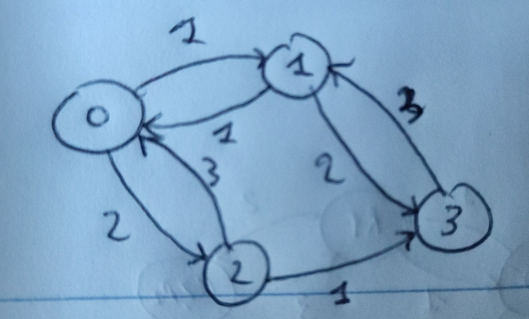
\includegraphics[width=10cm,height = 7cm]{img/srtategy1.png}
    \end{center}

    \caption{Strategy 1 : repairing machine 2 before machine 1}
    \label{label:markov}
\end{figure}

The stationary law is : $\pi = (\frac{6}{25},\frac{9}{25},\frac{3}{25},\frac{6}{25})$
For another stratedy which is repairing machine 1 before machine 2 :$\pi = (\frac{36}{91},\frac{12}{91},\frac{23}{91},\frac{20}{91})$ the markov chain is in the figure below : 
\begin{figure}[H]
    \begin{center}
        \includegraphics*[width = 10cm,height = 7cm]{img/strategy2.png}
    \end{center}
    \caption{Strategy 2, repairing machine 1 before machine 2}
\end{figure}

\textbf{a.} To maximize the time both machines we need to choose the strategy corresponding to $\pi_0$ is maximized which is strategy 2 as $\frac{36}{91} \ge \frac{6}{25}$.
\\\\
\textbf{b.} To minimize the time neither machine are working we choose the strategy that minimizes $\pi_3$ and it is strategy 1 that is to be prefered as $\frac{7}{25}\leq \frac{20}{91}$.
\\\\
\textbf{c.} The long run production rate can be computed as $\sum\limits_{i=0}^3\pi_i*\beta_i$ where $\beta_0 = \gamma_1+\gamma_2 = 5$, $\beta_1 = \gamma_2$, $\beta_2 = \gamma_1$ and $\beta_3 = 0$. $$\boxed{\text{The strategy that maximizes the long-run production rate is Strategy 2, repairing machine 1 before machine 2.}}$$
\section*{Additional Problem 2 :}
As $m(t) = \frac{t}{2}$ then $1 = 2F'(t)+F(t)$ which is a differencial equation and solutions of this equations are $s\in \text{Vect}(e^{-\frac{t}{2}})+1$. With the conditions $F(0) = 0$ and $\lim_{t\to\infty}F(t) = 1$ we have $F(t) = 1-e^{-\frac{t}{2}}$.
$$\boxed{\mathbb{P}(N(5) = 0) = 1-F(5) = e^{-\frac{5}{2}}}$$ 
\end{document}
